\section{Virtual indoor mapping generation workflow}\label{workflow}


\begin{figure*}[ptb] %  figure placement: here, top, bottom, or page
   \centering
   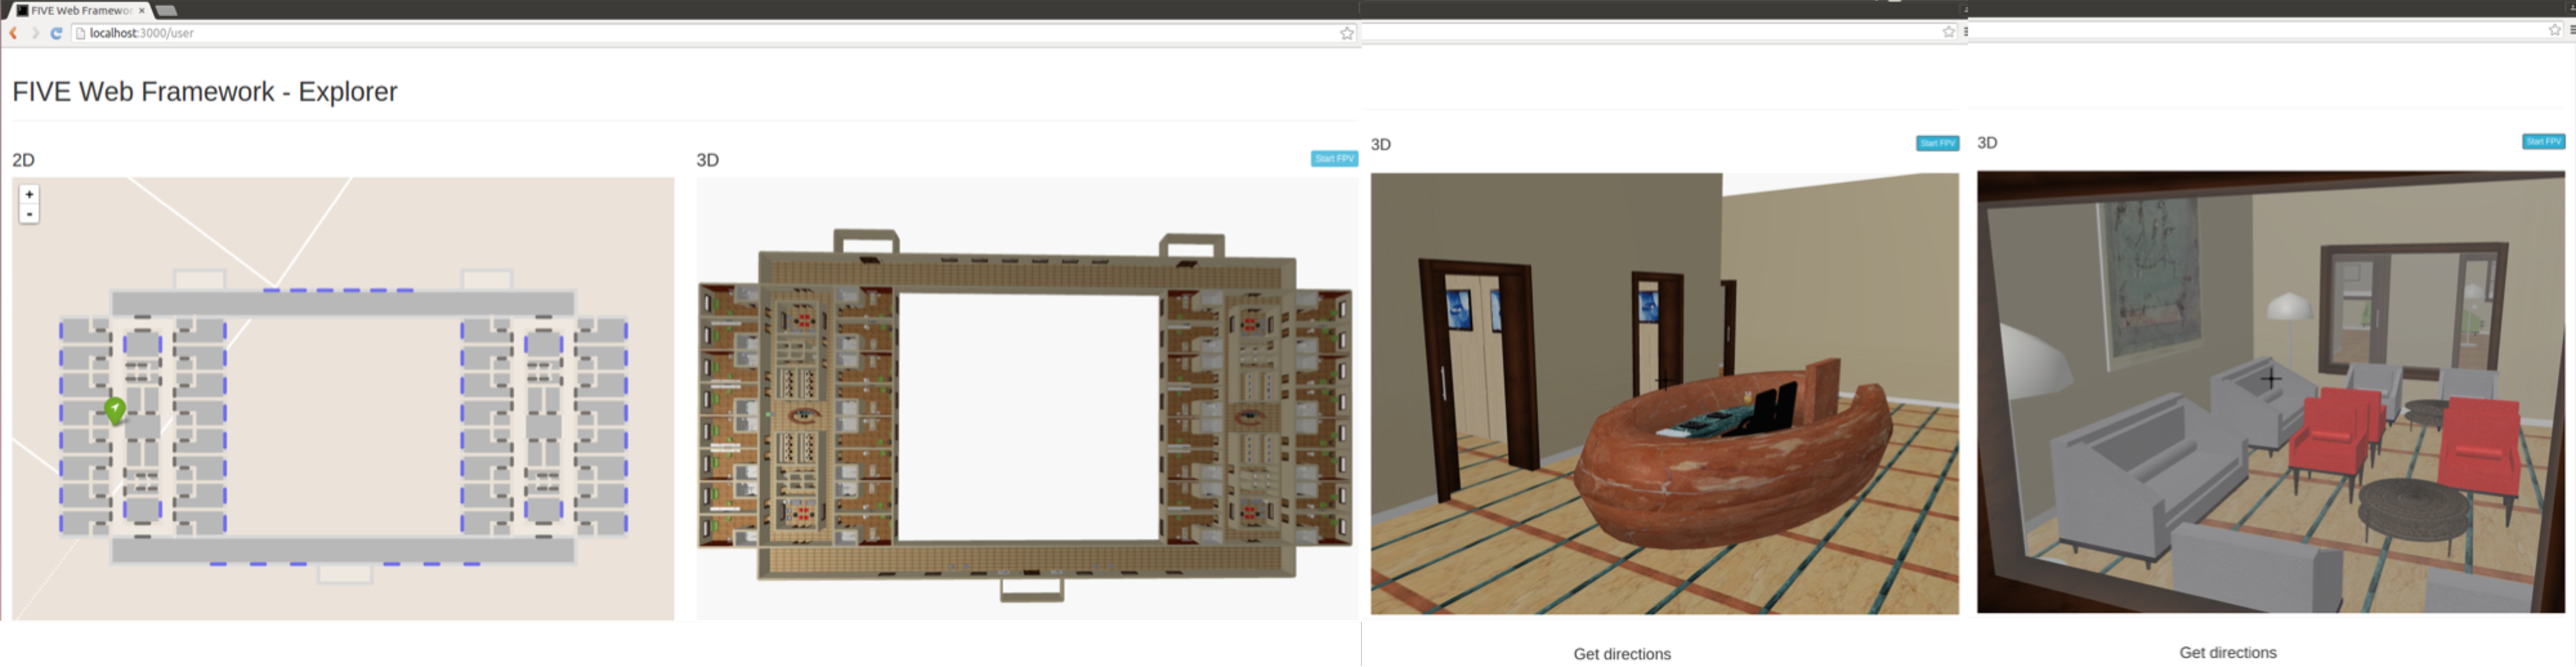
\includegraphics[width=\linewidth]{images/ward/ward} 
   
   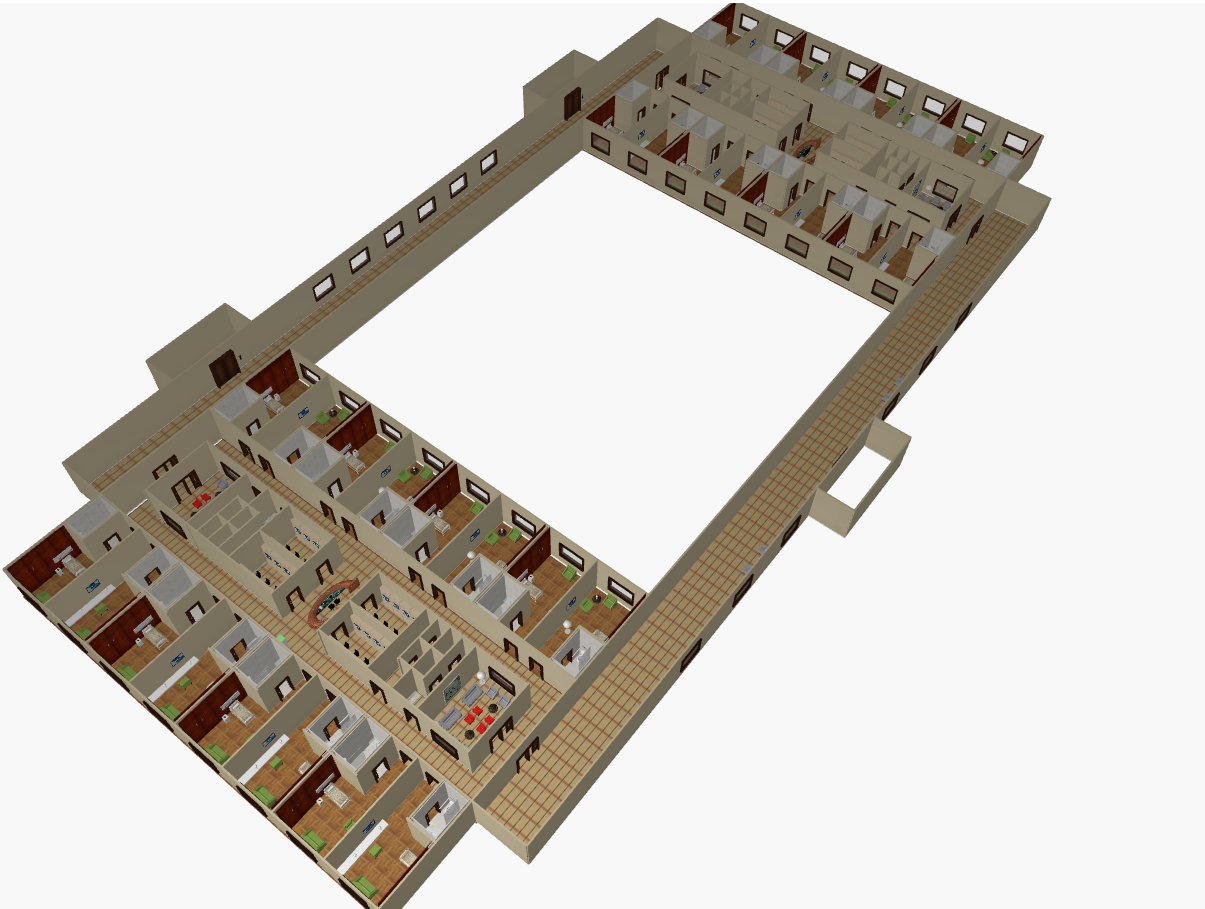
\includegraphics[width=0.327\linewidth]{images/ward/ward1} 
   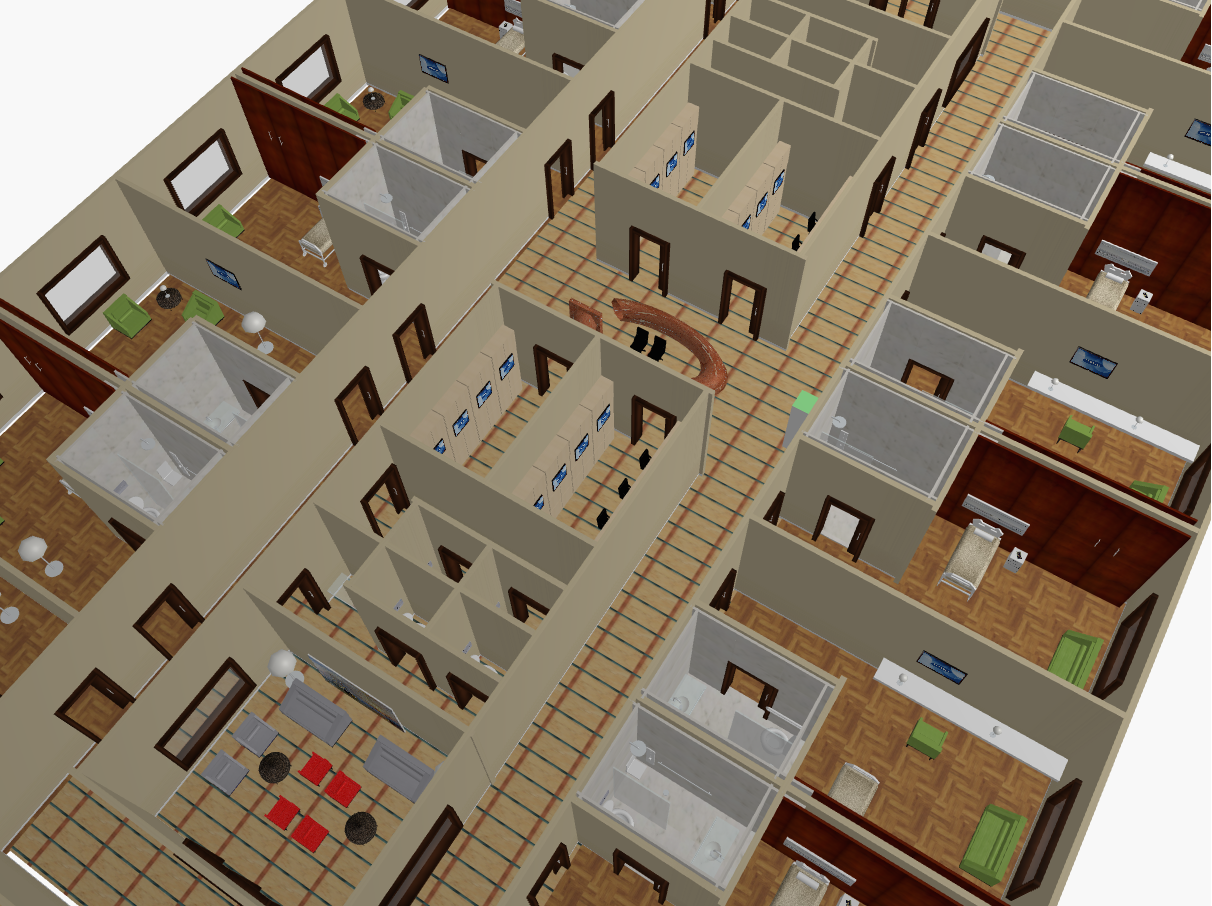
\includegraphics[width=0.327\linewidth]{images/ward/ward4} 
   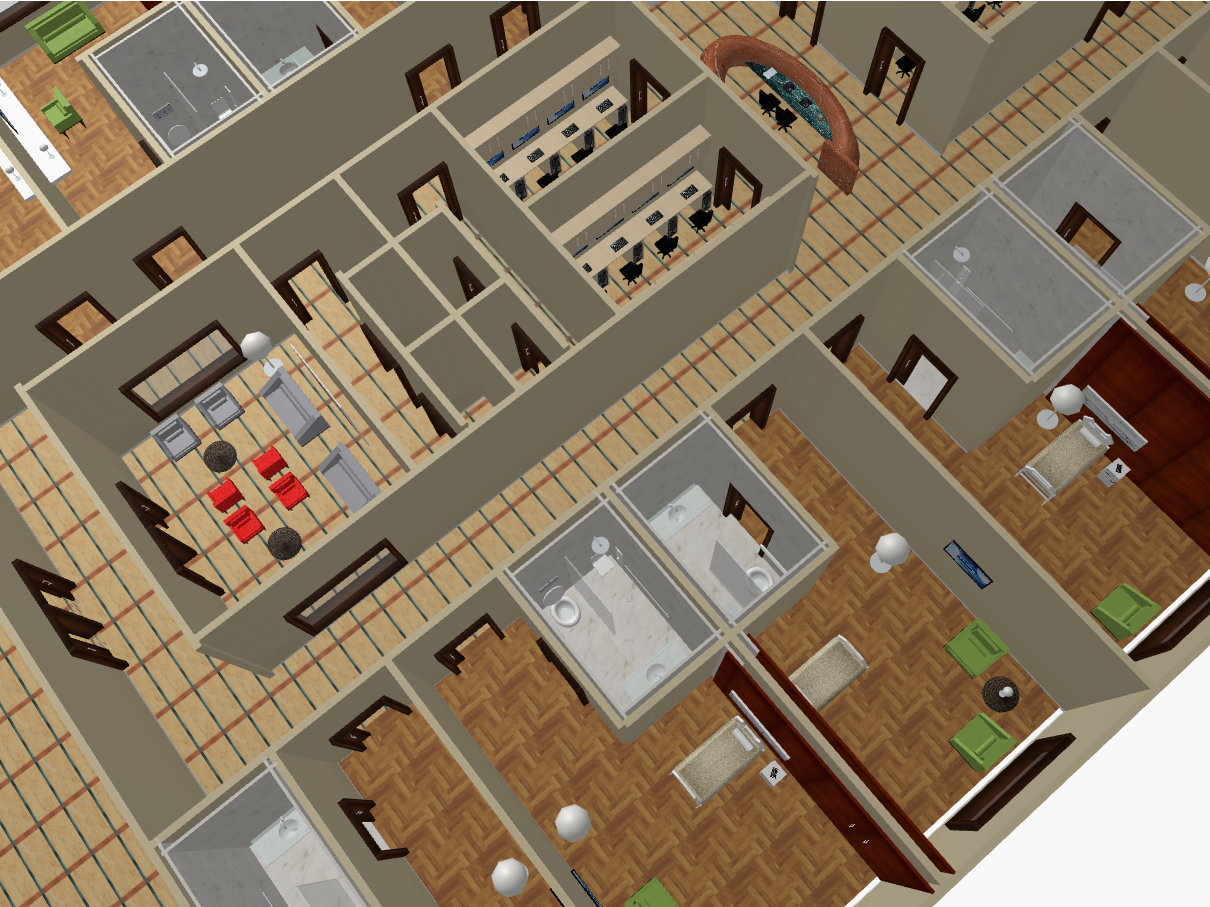
\includegraphics[width=0.327\linewidth]{images/ward/ward5} 
   \caption{Some images of two ward departments of an hospital design from an interactive session with the FIVE environment.}
   \label{fig:example}
\end{figure*}



\begin{figure*}[ptb] %  figure placement: here, top, bottom, or page
   \centering
   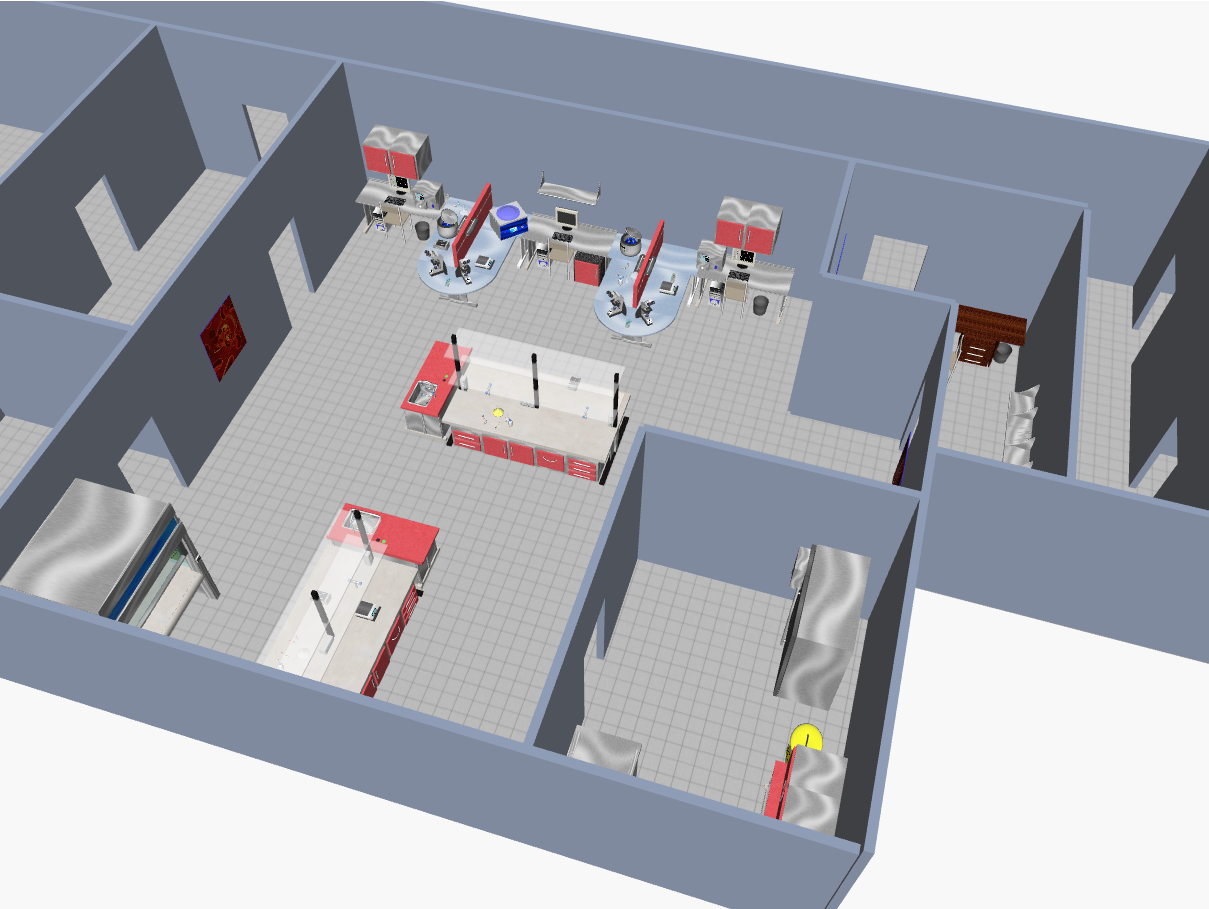
\includegraphics[width=0.327\linewidth]{images/lab/lab0} 
   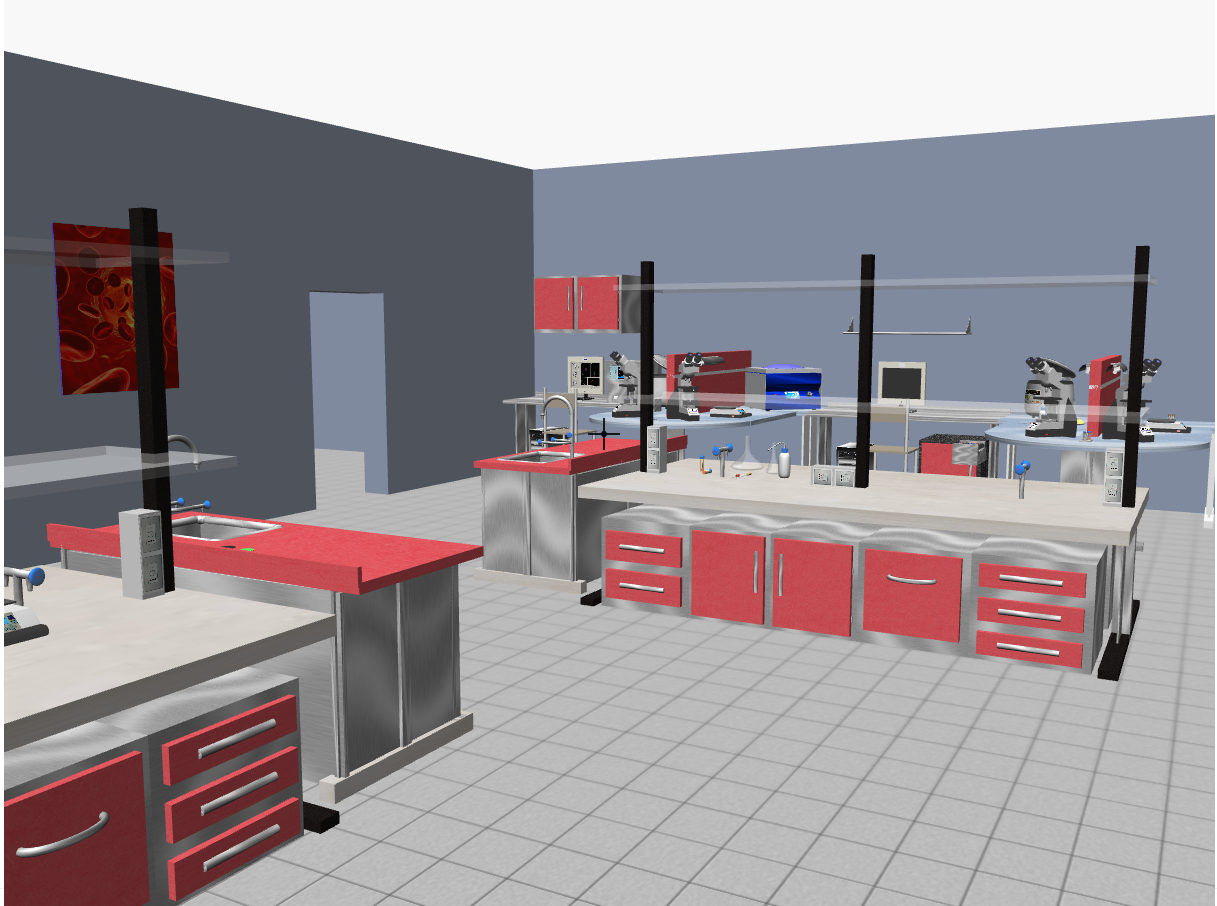
\includegraphics[width=0.327\linewidth]{images/lab/lab2} 
   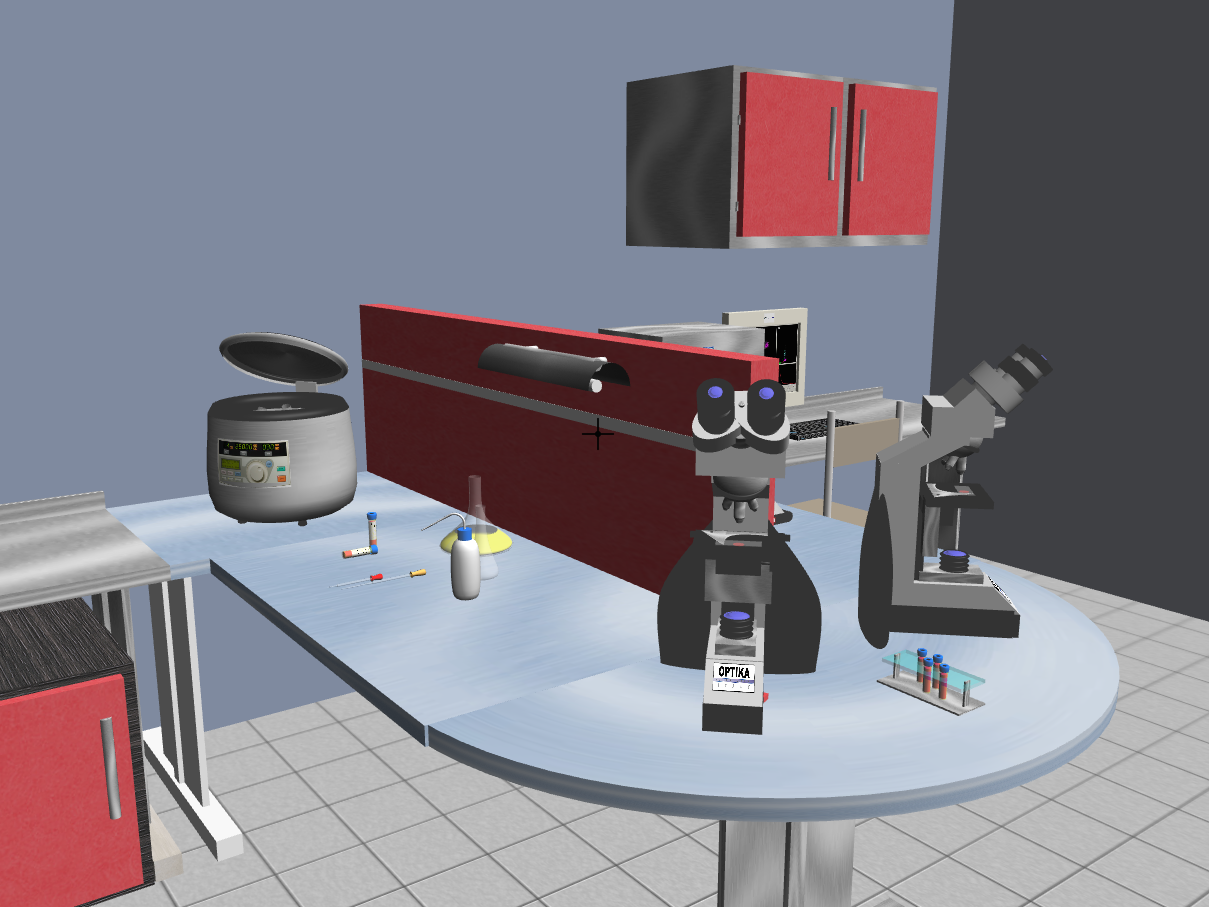
\includegraphics[width=0.327\linewidth]{images/lab/lab3} 

   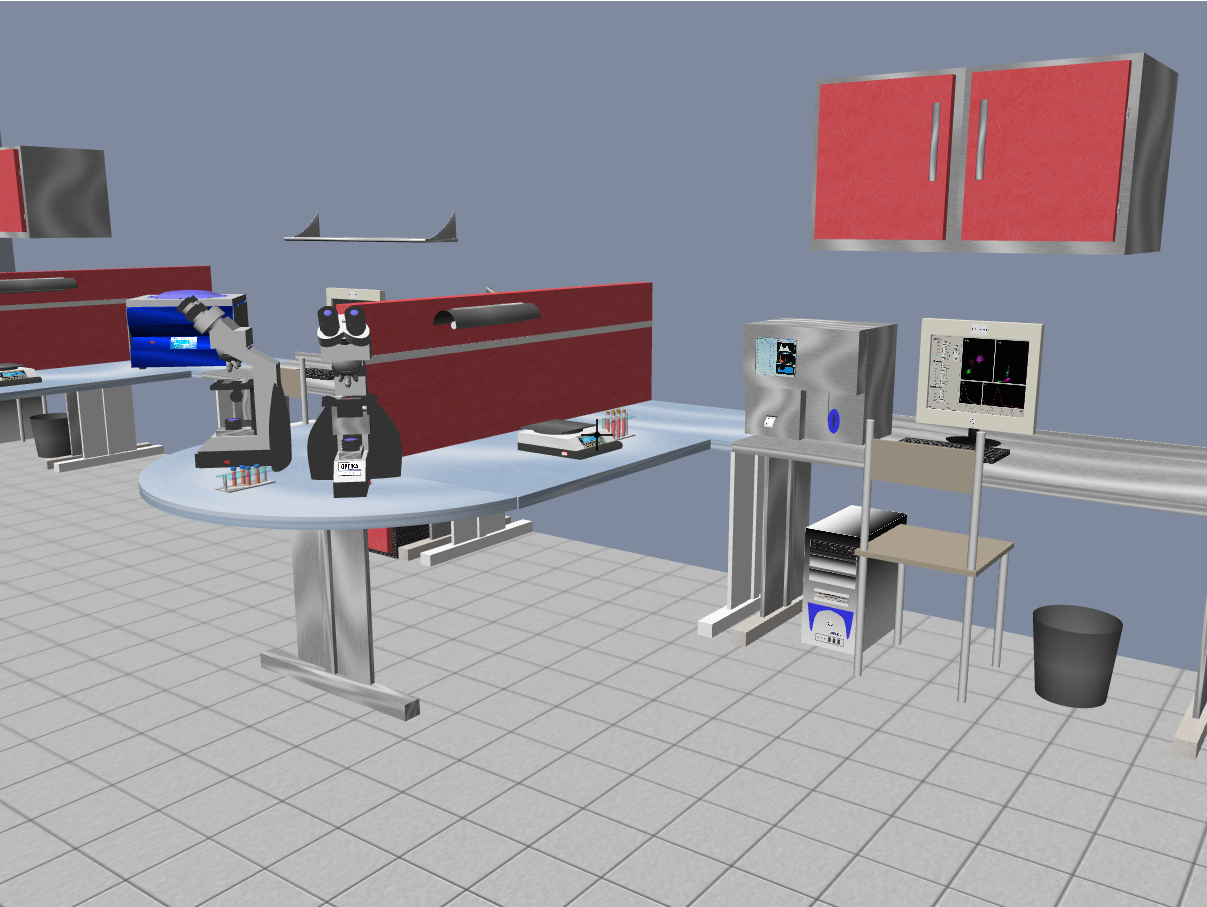
\includegraphics[width=0.327\linewidth]{images/lab/lab4} 
   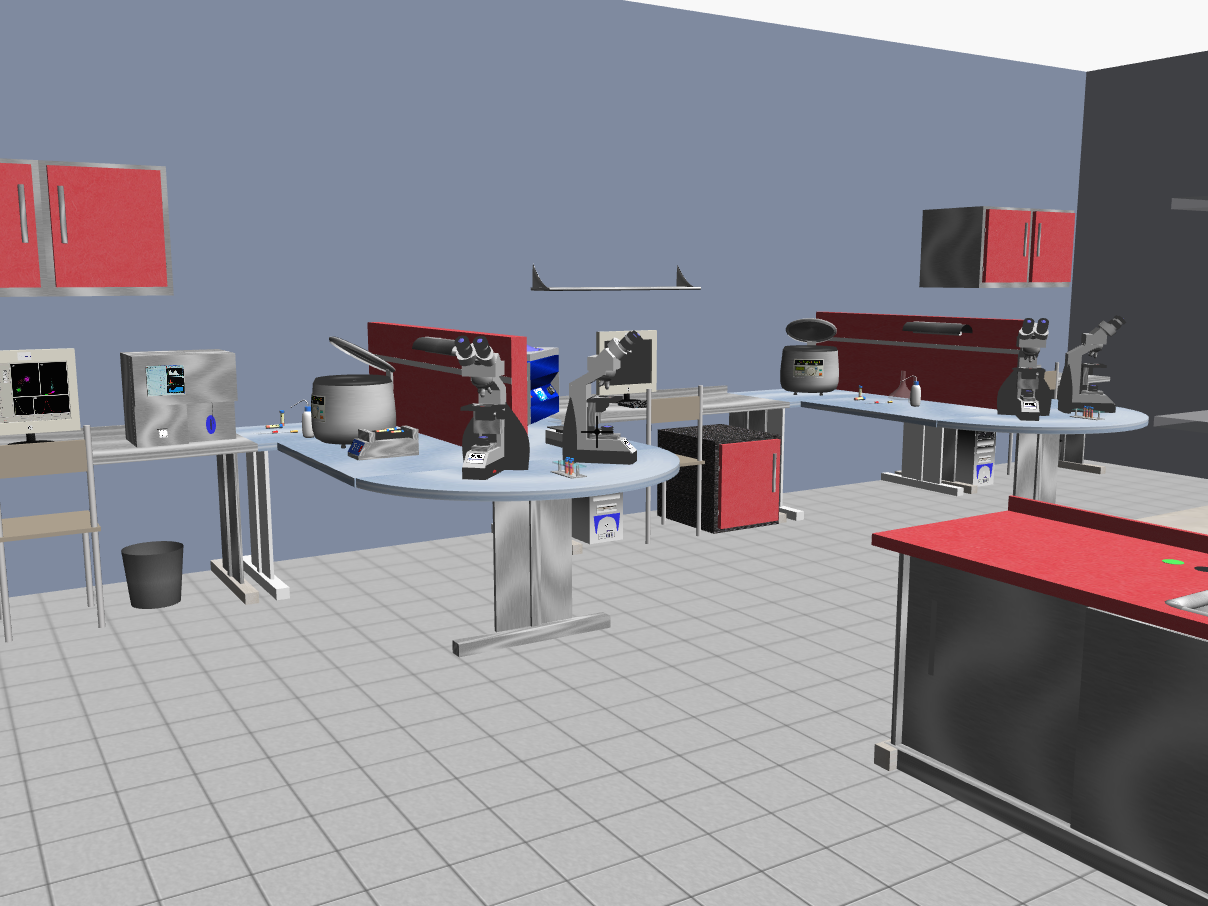
\includegraphics[width=0.327\linewidth]{images/lab/lab5} 
   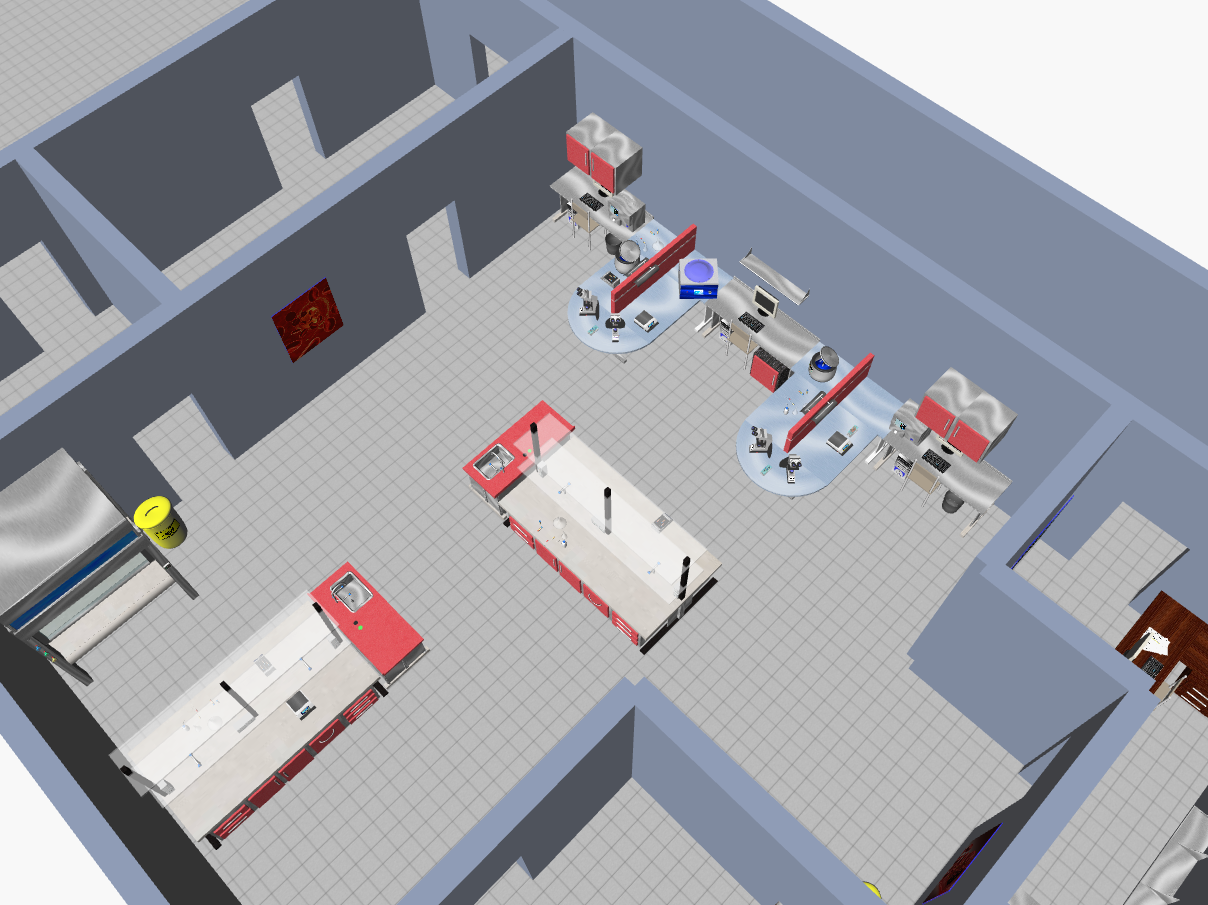
\includegraphics[width=0.327\linewidth]{images/lab/lab6} 
   \caption{Some images of the Laboratories department of an hospital design.}
   \label{fig:example}
\end{figure*}


\begin{figure}[ptb] % figure placement: here, top, bottom, or page
 \centering
 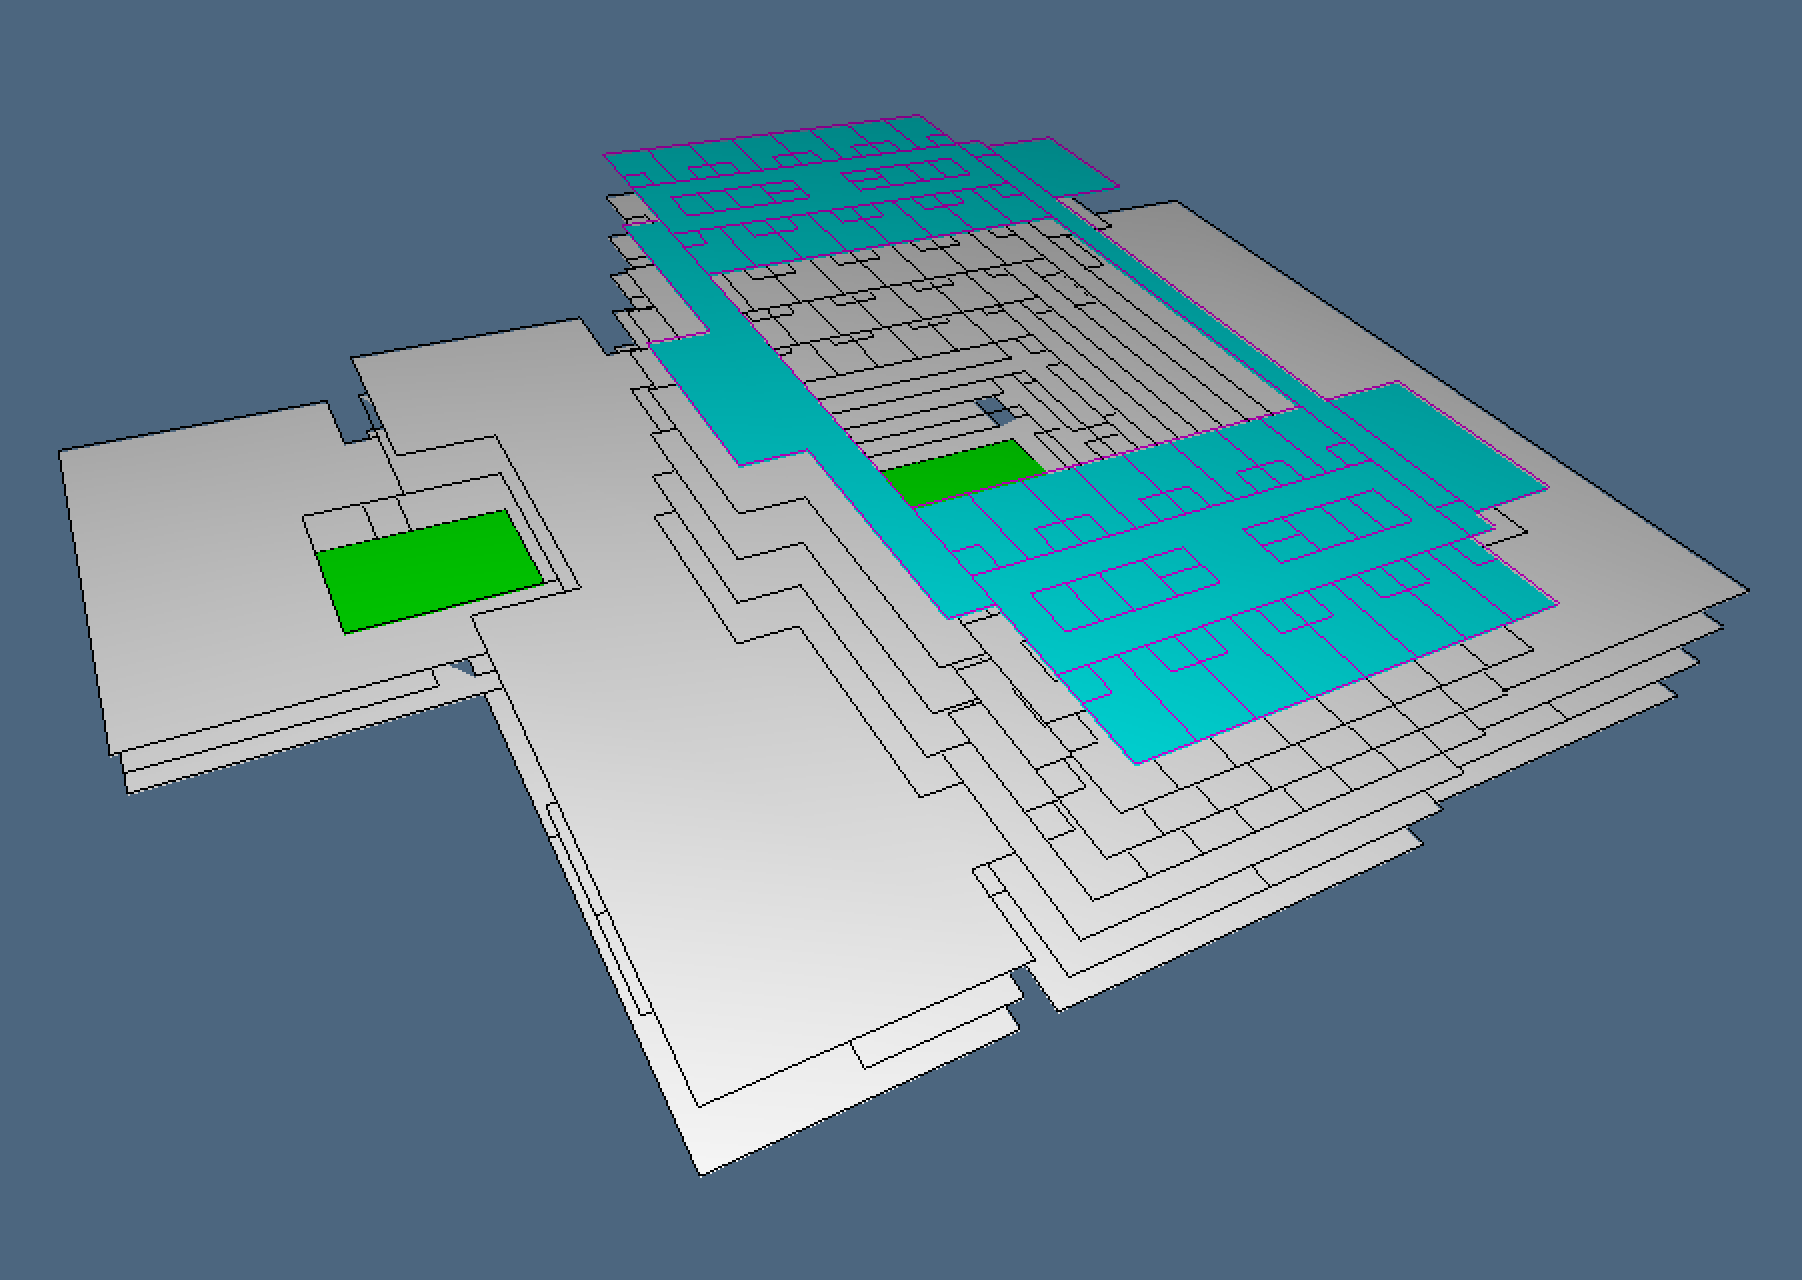
\includegraphics[width=\linewidth]{images/hospital2} 
 \caption{An image of the 2.5D model of a general hospital, defined as the LAR of a 2-complex embedded in 3-space. Notice that 2-cells may be non-convex. The cyan floor corresponds the pair of ward departments translated into the HIJSON format and displayed in the previous pages.}
 \label{fig:hospital2}
\end{figure}

The 2.5D model of the built environment to interact with is generated offline and server-side, finally producing a HIJSON format. This  files are served on the web and transformed real-time client-side into the FIVE interactive interface (either 2D, or 3D or both) of the indoor mapping applications. The sequence of steps is outlined below:

1. \textit{Input of wire-frame drawings},
  starting from architectural  raster \emph{images} of building floorplans, interpreted into a simplified 2D vector representation (\texttt{.svg} files);

2. \textit{Generation of a 2D cellular complex}, via
  parsing of graphics elements from textual files, and automatic generation of a 2D cellular complex for topological computations and long-term storage of the model (\texttt{.lar} files) using a very simple and general geometric format (LAR) based on algebraic topology and linear algebra with compressed sparse matrices;

3. \textit{Structured 2.5D description}, produced by
  hierarchical modeling of cellular models, through automatic transformation of  grouping elements of \texttt{.svg} files into a 2D description providing \emph{semantics} to spaces and  to the various elements of the building fabric (vertical or horizontal external envelope, internal partitions, horizontal floors, vertical communications), by using an object-oriented hierarchical description as a  \texttt{Struct} network;

4. \textit{Exporting to HIJSON file}.
The  structured and semantically annotated 2.5D building model is finally  exported as a rich textual description into \texttt{HIJSON} files, i.e.~in JSON format, though and intermediate \texttt{.yml} translation;

5. \textit{Client-based processing}
  The \texttt{.json} files are finally transformed client-side into both
  2D and 3D environments allowing the real-time spatial placement and
  user-tracing within the virtual environment of the individuals moving
  inside the real building.

